\section{Obtención de velocidad}

Como se mencionó anteriormente en la Sección \ref{cap:metodologia} la obtención de la velocidad se divide en tres partes las cuales están representadas en el Figura \ref{fig:DFObtencionDeVelocidad} y se describen a continuación.

\begin{figure}[H]
    \centering
    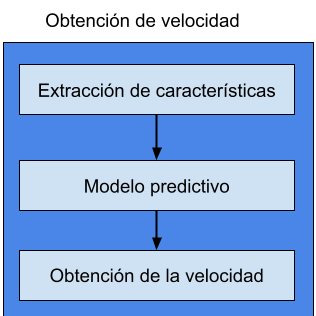
\includegraphics[width=0.5\textwidth]{Metodologia/imgs/ObtencionVelocidad.png}
    \caption{Proceso de obtención de velocidad.}
    \label{fig:DFObtencionDeVelocidad}
\end{figure}

\subsection{Extracción de características }

En el paso anterior para cada muestra se creo un archivo csv el cual servirá de entrada para el paso actual.

El sistema se encarga de leer el video utilizando la biblioteca OpenCV con la cual se extraen los fotogramas del video, cada fotograma pasa por la red neuronal YOLO la cual se encarga de identificar todos los vehículos que aparecen en el fotograma. YOLO regresa las coordenadas de cada objeto detectado dentro del fotograma, estas coordenadas son usadas para dibujar un recuadro para cada objeto. La Figura \ref{fig:LugarDeteccion} muestra dos vehículos detectados.

\begin{figure}[H]
    \centering
    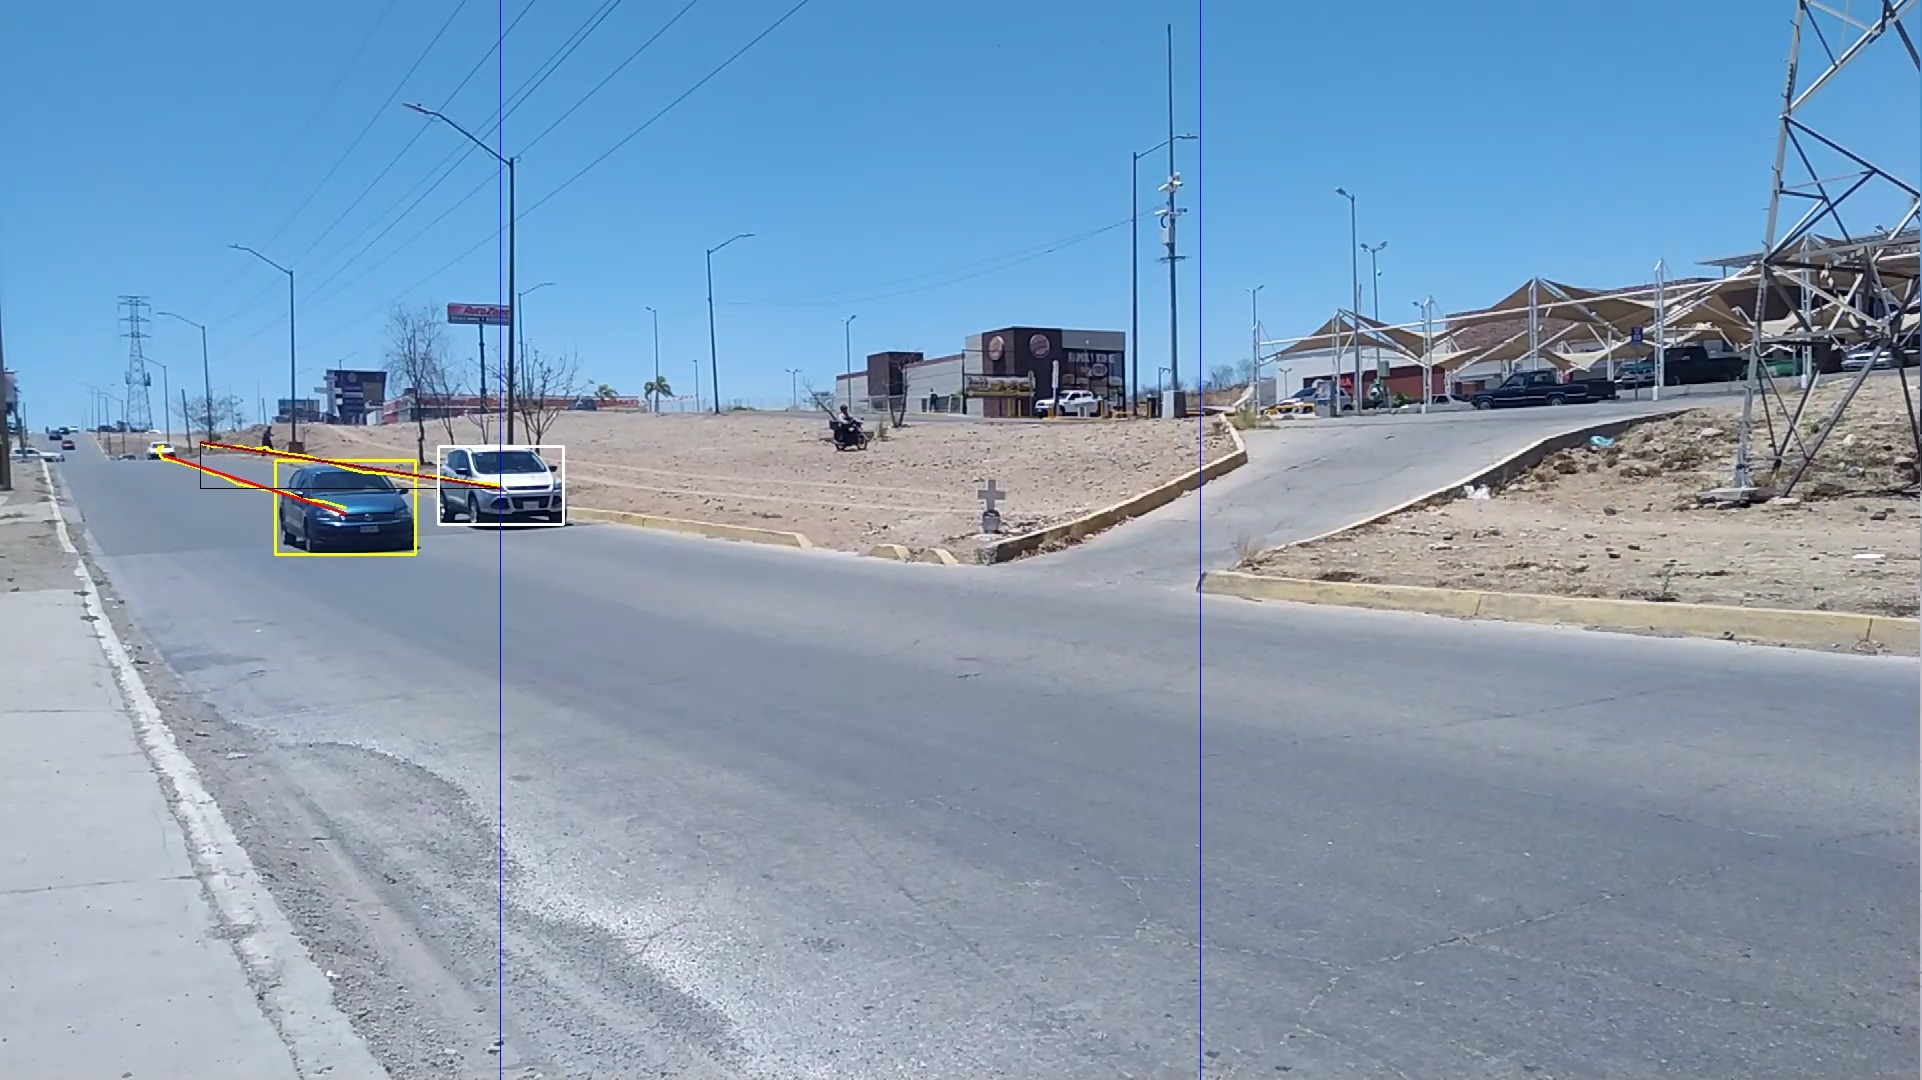
\includegraphics[width=0.8\textwidth]{Metodologia/imgs/Deteccion.jpg}
    \caption{Detección de vehículos dentro de recuadros.}
    \label{fig:LugarDeteccion}
\end{figure}

El seguimiento de los vehículos se realiza por medio del Filtro Kalman el cual determina su ubicación en el próximo fotograma. El sistema se encarga de guardar todas las ubicaciones de los vehículos en el transcurso del tiempo siendo capaz dibujar todo el trayecto que han tenido cada uno de ellos. Sumando el uso de regresión lineal se crea una recta que corresponde a las trayectorias de los vehículos. La Figura \ref{fig:LugarSeguimiento} muestra un vehículo detectado en un recuadro blanco, una línea amarilla con la trayectoria del vehículo y una línea roja la cual es generada con regresión a partir de la trayectoria del vehículo.

\begin{figure}[H]
    \centering
    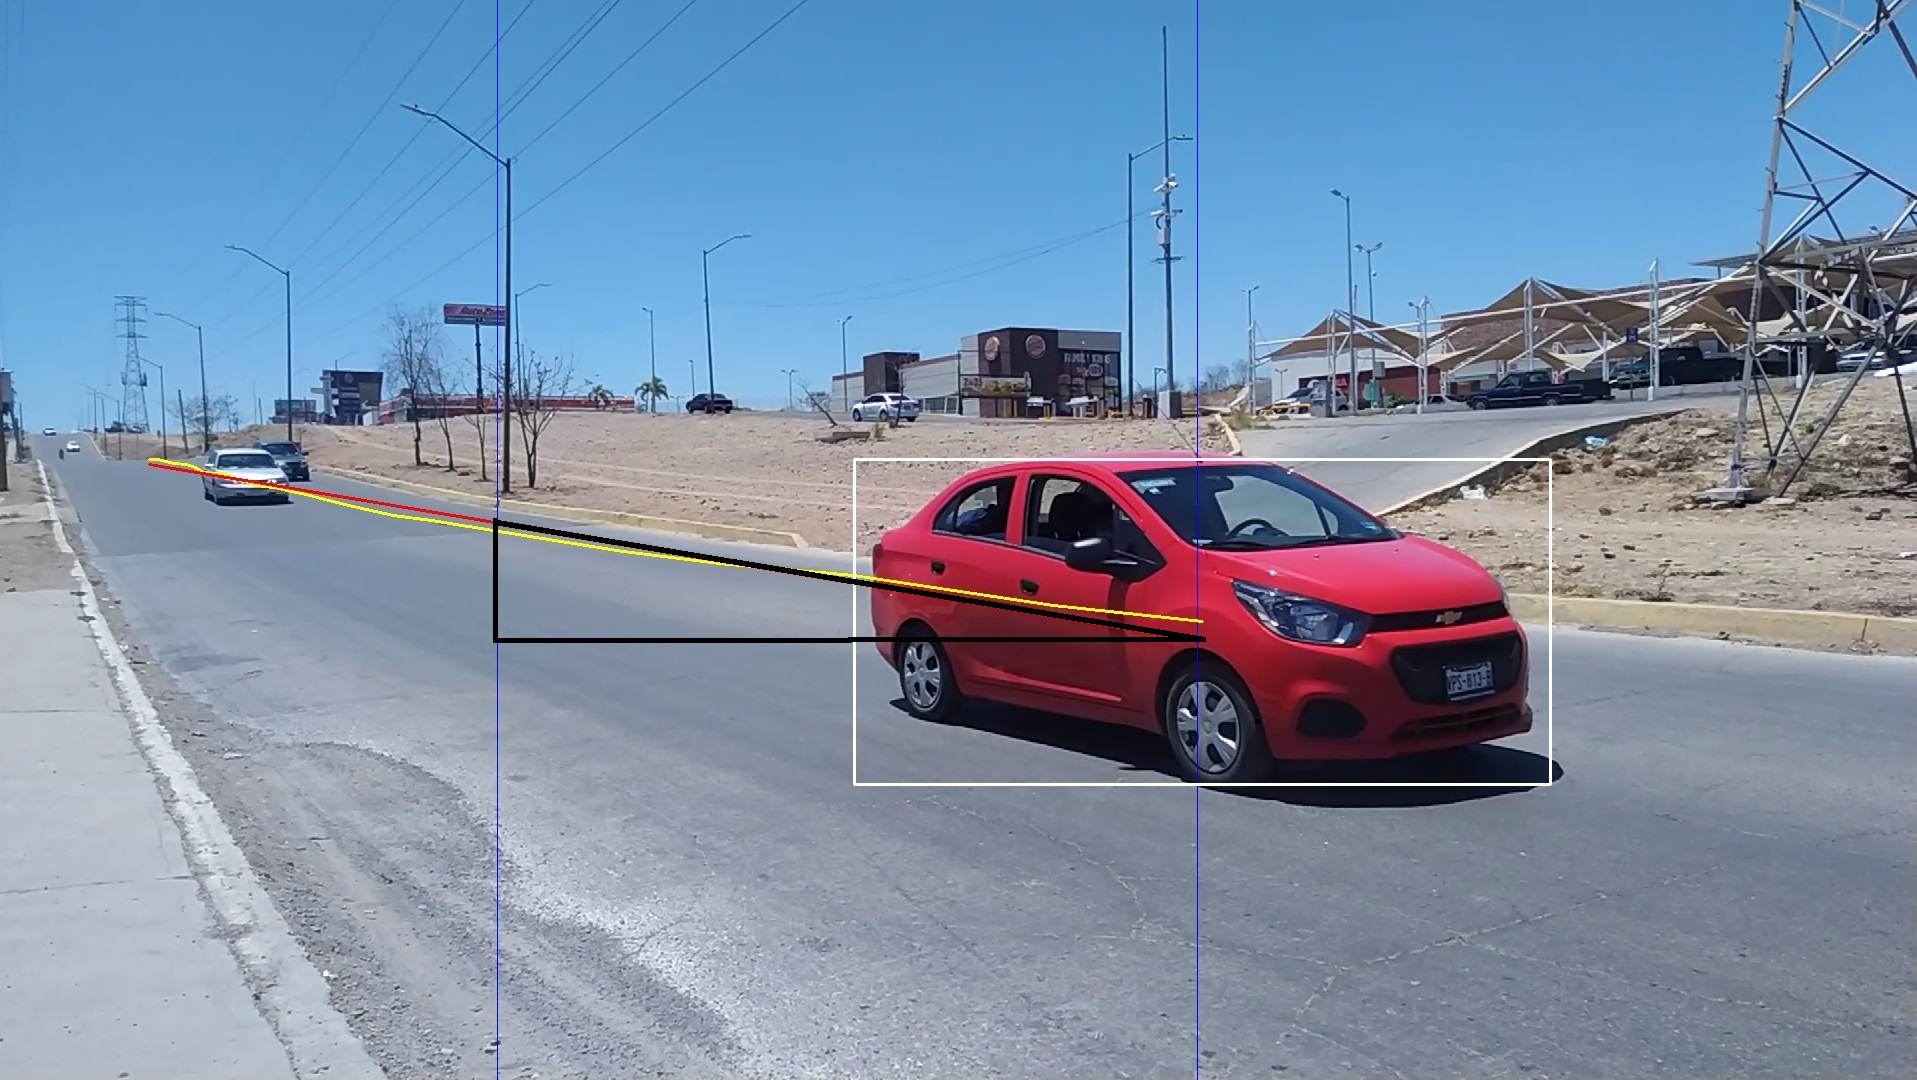
\includegraphics[width=0.8\textwidth]{Metodologia/imgs/Seguimiento_01.jpg}
    \caption{Detección de vehículos en punto B, sus trayectorias y triangulación del generado con el punto A y B.}
    \label{fig:LugarSeguimiento}
\end{figure}

Otra característica que se identifica en la Figura \ref{fig:LugarSeguimiento} es la creación de un triángulo en color negro, con el cual se identifica el ángulo detectado para el vehículo.

Cando el sistema detecta que un vehículo pasa por el punto A, este guarda la información del estado del vehículo (Figura \ref{fig:PuntoA}). Puede haber múltiples vehículos pasando en ese momento y todos serán detectados por el sistema. El vehículo del cual se obtienen sus características esta identificado con un recuadro de color amarillo, mientras que el resto de los vehículos están dentro de un recuadro color amarillo.


\begin{figure}[H]
    \centering
    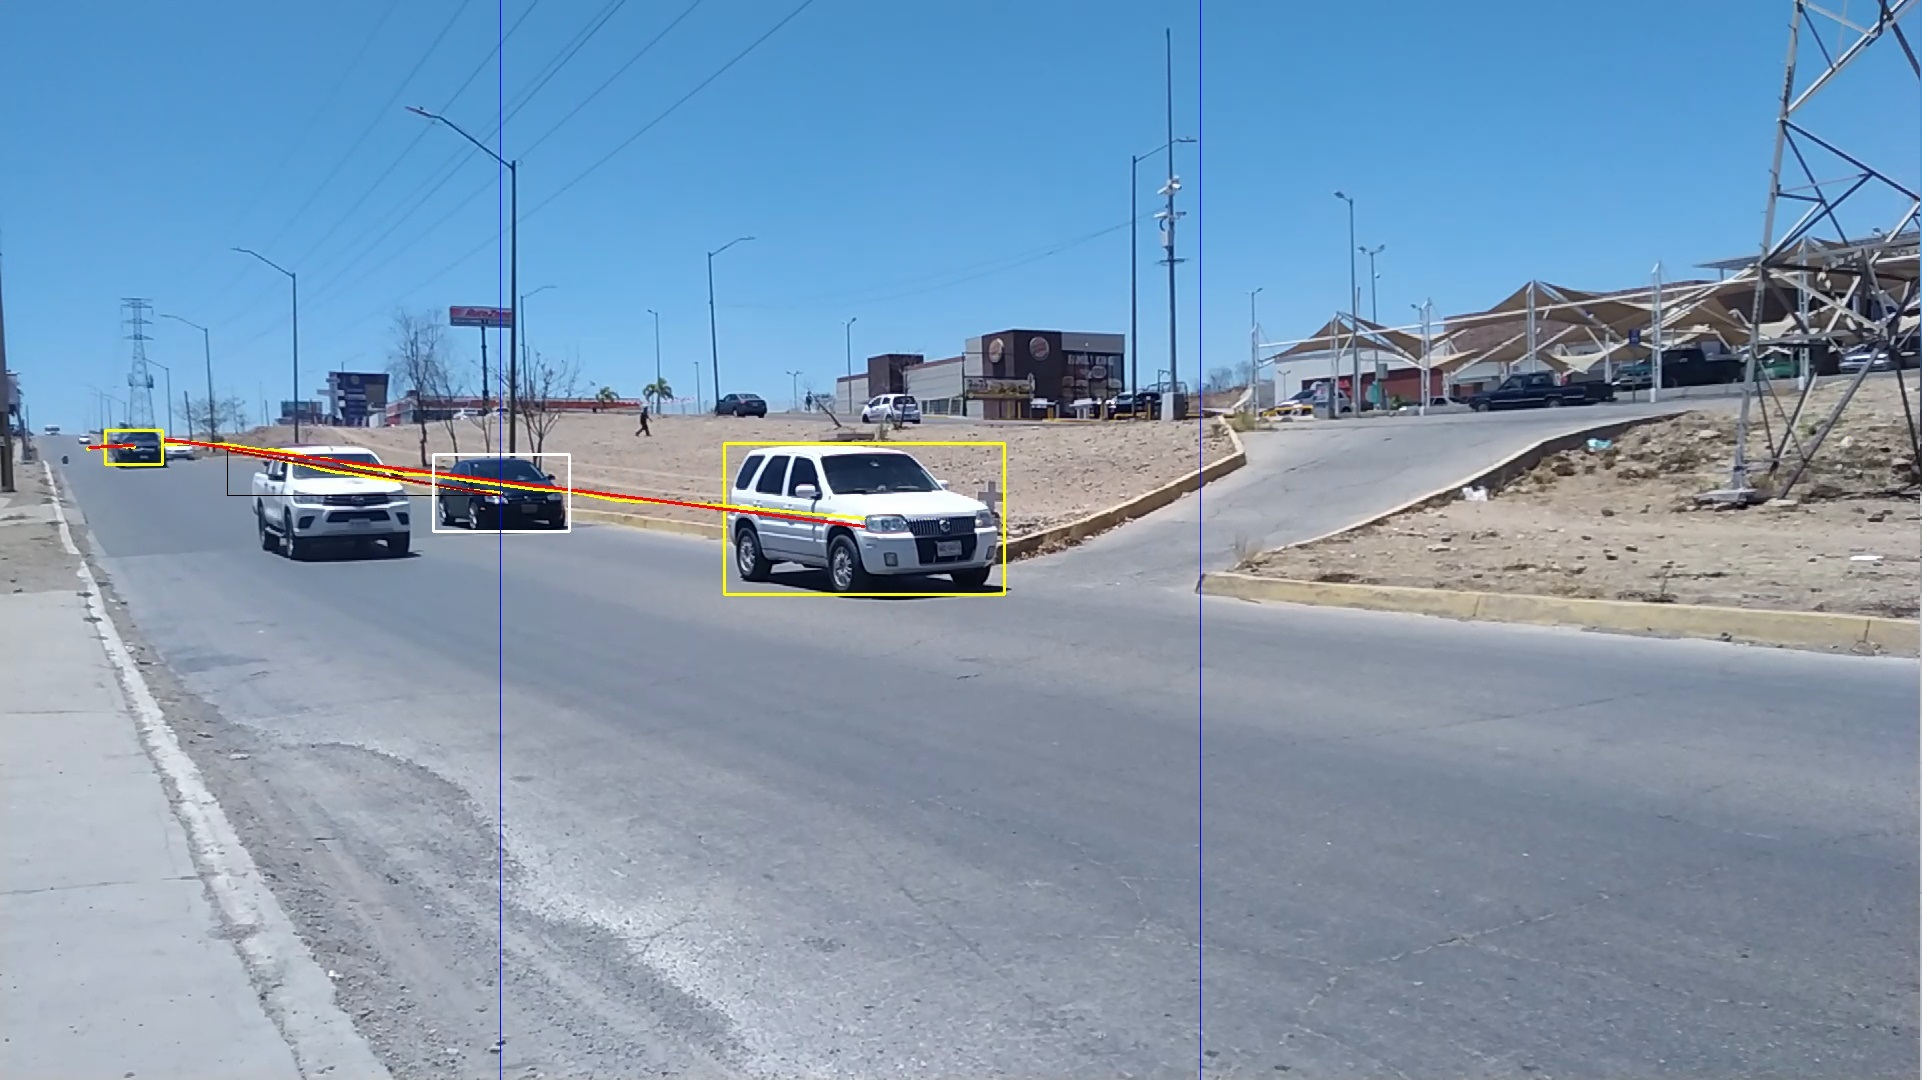
\includegraphics[width=0.8\textwidth]{Metodologia/imgs/Punto_A.jpg}
    \caption{Punto A con vehículo en recuadro blanco.}
    \label{fig:PuntoA}
\end{figure}

Aunque se guardó el estado del vehículo cuando paso por el punto A, este no genera una línea para el archivo csv resultante. Es hasta que el vehículo pasa por el punto B y coincide con los segundos en el archivo csv de entrada que el sistema guarda un nuevo dato en el archivo de salida. Los vehículos que no cuentan con una línea en el archivo csv de entrada no se les guarda su información. La Figura \ref{fig:PuntoB} muestra cuando el vehículo detectado en el punto A pasa por el punto B.

\begin{figure}[H]
    \centering
    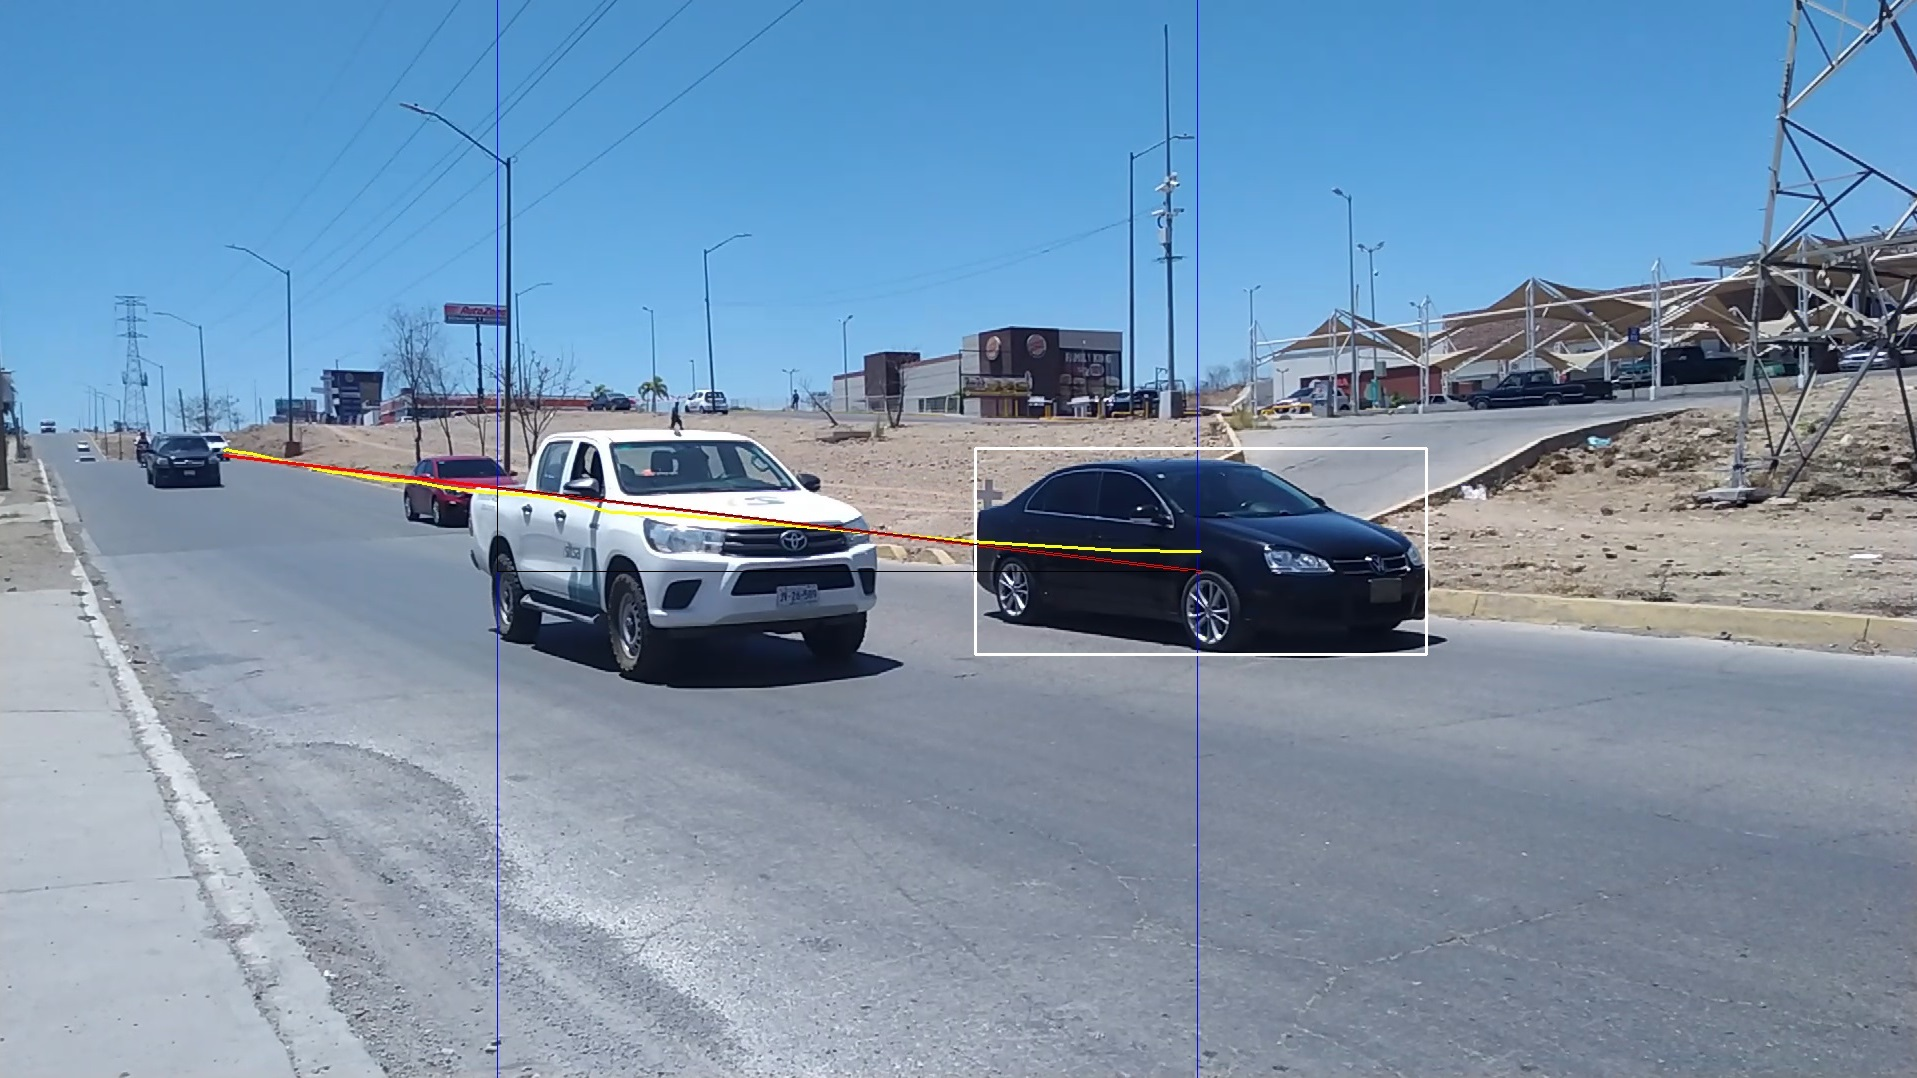
\includegraphics[width=0.8\textwidth]{Metodologia/imgs/Punto_B.jpg}
    \caption{Punto B con vehículo en recuadro blanco.}
    \label{fig:PuntoB}
\end{figure}

La Tabla \ref{tab:CaracteristicasSistema} muestra las características más importante que son extraídas por el sistema y una descripción.

\begin{table}[H]
    \caption{Características obtenidas por el sistema.}
    \label{tab:CaracteristicasSistema}
    \begin{tabular}{|l|l|}
        \hline
        \textbf{Característica} & \multicolumn{1}{c|}{\textbf{Descripción}} \\ \hline
        \textbf{Ángulo Salida} & Ángulo a partir del punto de entrada hasta el punto de salida \\ \hline
        \textbf{Distancia de salida} & Distancia recorrida desde el punto de entrada hasta el punto de salida \\ \hline
        \textbf{Área Entrada} & Área detectada del vehículo en pixeles en el punto de entrada \\ \hline
        \textbf{Área Salida} & Área detectada del vehículo en pixeles en el punto de salida \\ \hline
        \textbf{FPS} & Fotogramas por segundo del video \\ \hline
        \textbf{Tiempo} & Tiempo que le tomo al vehículo para pasar del punto entrada al de salida \\ \hline
        \textbf{Velocidad} & Velocidad detectada por el radar \\ \hline
        \textbf{Carril} & Carril por que pasa el vehículo \\ \hline
        \textbf{Identificador} & Identificador correspondiente a una imagen generada \\ \hline
    \end{tabular}
\end{table}


El sistema además de generar un archivo csv, crea una imagen de salida la cual corresponde a una línea del archivo resultante, esta imagen está formada por dos imágenes una al lado de la otra, la imagen de la izquierda representa el vehículo cuando entra en el punto A y la imagen de la derecha es cuando el vehículo pasa por el punto B. La Figura \ref{fig:Completo} muestra un ejemplo de esta imagen de salida.

\begin{figure}[H]
    \centering
    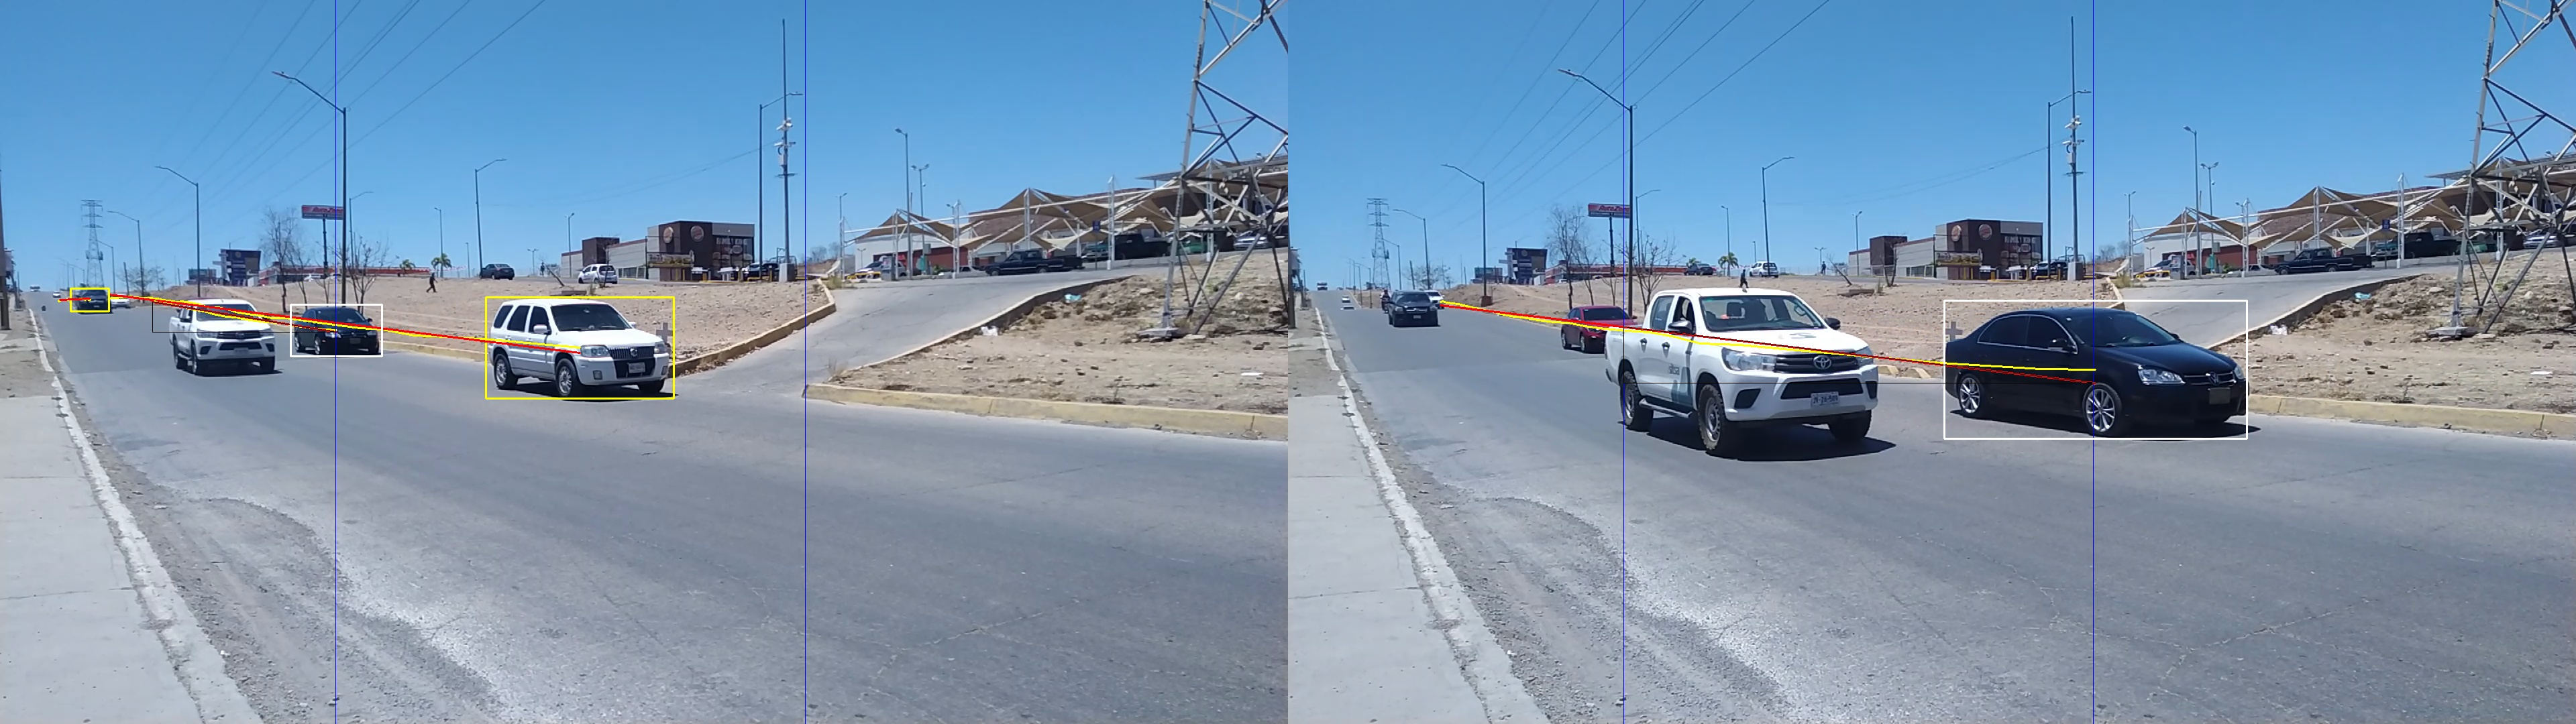
\includegraphics[width=1\textwidth]{Metodologia/imgs/Completo.jpg}
    \caption{Imagen resultado para cada línea de archivo csv.}
    \label{fig:Completo}
\end{figure}

%%%%%%%%%%%%%%%%%%%%%%%%%%%%%%%%%%%%%%%%%%%%%%%%%%%%%%%%%%%%%%%%%%%%%%%%%%%%%%%%
%%%%%%%%%%%%%%%%%%%%%%%%%%%%%%%%%%%%%%%%%%%%%%%%%%%%%%%%%%%%%%%%%%%%%%%%%%%%%%%%
%%%%%%%%%%%%%%%%%%%%%%%%%%%%%%%%%%%%%%%%%%%%%%%%%%%%%%%%%%%%%%%%%%%%%%%%%%%%%%%%
%%%%%%%%%%%%%%%%%%%%%%%%%%%%%%%%%%%%%%%%%%%%%%%%%%%%%%%%%%%%%%%%%%%%%%%%%%%%%%%%
%%%%%%%%%%%%%%%%%%%%%%%%%%%%%%%%%%%%%%%%%%%%%%%%%%%%%%%%%%%%%%%%%%%%%%%%%%%%%%%%

Una vez que el sistema genera las imágenes de salida. El archivo csv resultante valida que el vehículo detectado sea el correcto y que el recuadro blanco que define la detección del vehículo contenga la mayor parte del vehículo.

Para el caso de validar que el vehículo sea el correcto, es necesario ver cada una de las imágenes generadas y leer la descripción en el archivo csv de entrada. En caso de identificar un vehículo que no corresponda, se debe modificar los segundos en el archivo csv de entrada de tal manera que el sistema detecte el vehículo  correcto, esto implica ejecutar el sistema nuevamente para generar los datos de nuevo. 

Existen dos casos en los que el sistema no podrá identificar el vehículo. El primer caso implica que el vehículo sea obstaculizado por otro. Por lo cual, la detección será del vehículo que esta frente al vehículo que se le esta realizando el seguimiento. El segundo caso corresponde cuando al vehículo no se le realizo el seguimiento completo del punto A al B de forma correcta, esto implica que el vehículo no fue detectado en el camino. Para estos dos caso se elimina la línea correspondiente en el archivo de entrada, lo cual también implica ejecutar el sistema nuevamente para generar los datos nuevamente.


Para validar que el área de detección del vehículo sea completa, se realizó una inspección visual de las imágenes generadas. Durante la inspección se identifica
el vehículo cuando entra en el punto A (Figura \ref{fig:ImagenValida01}) el cual debe ser detectado completamente por el recuadro blanco, al mismo tiempo que se identifica el vehículo cuando pasa por el punto B (Figura \ref{fig:ImagenValida02}) el cual también debe ser identificado completamente por el recuadro blanco.


\begin{figure}[H]
    \centering
    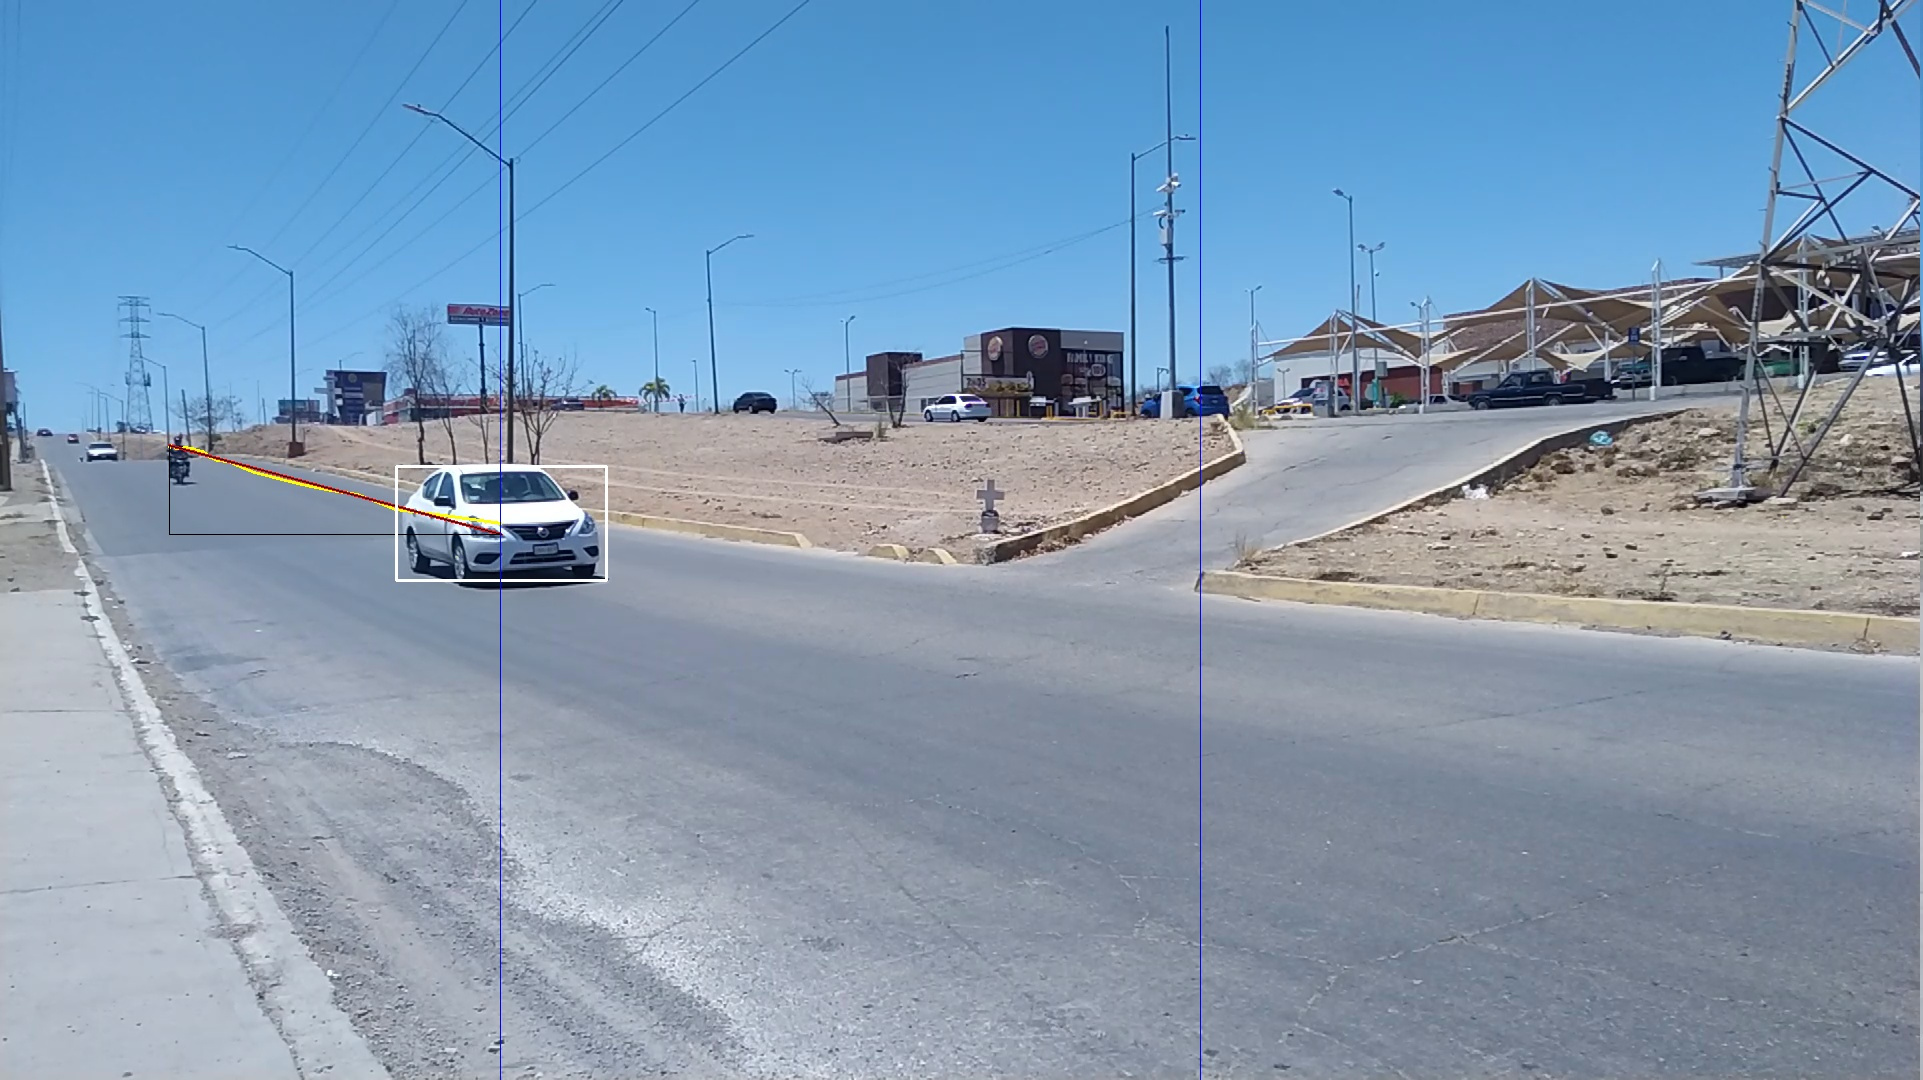
\includegraphics[width=0.8\textwidth]{Metodologia/imgs/Valido_001.jpg}
    \caption{Imagen válida con vehículo entrando representando una línea del archivo csv.}
    \label{fig:ImagenValida01}
\end{figure}

\begin{figure}[H]
    \centering
    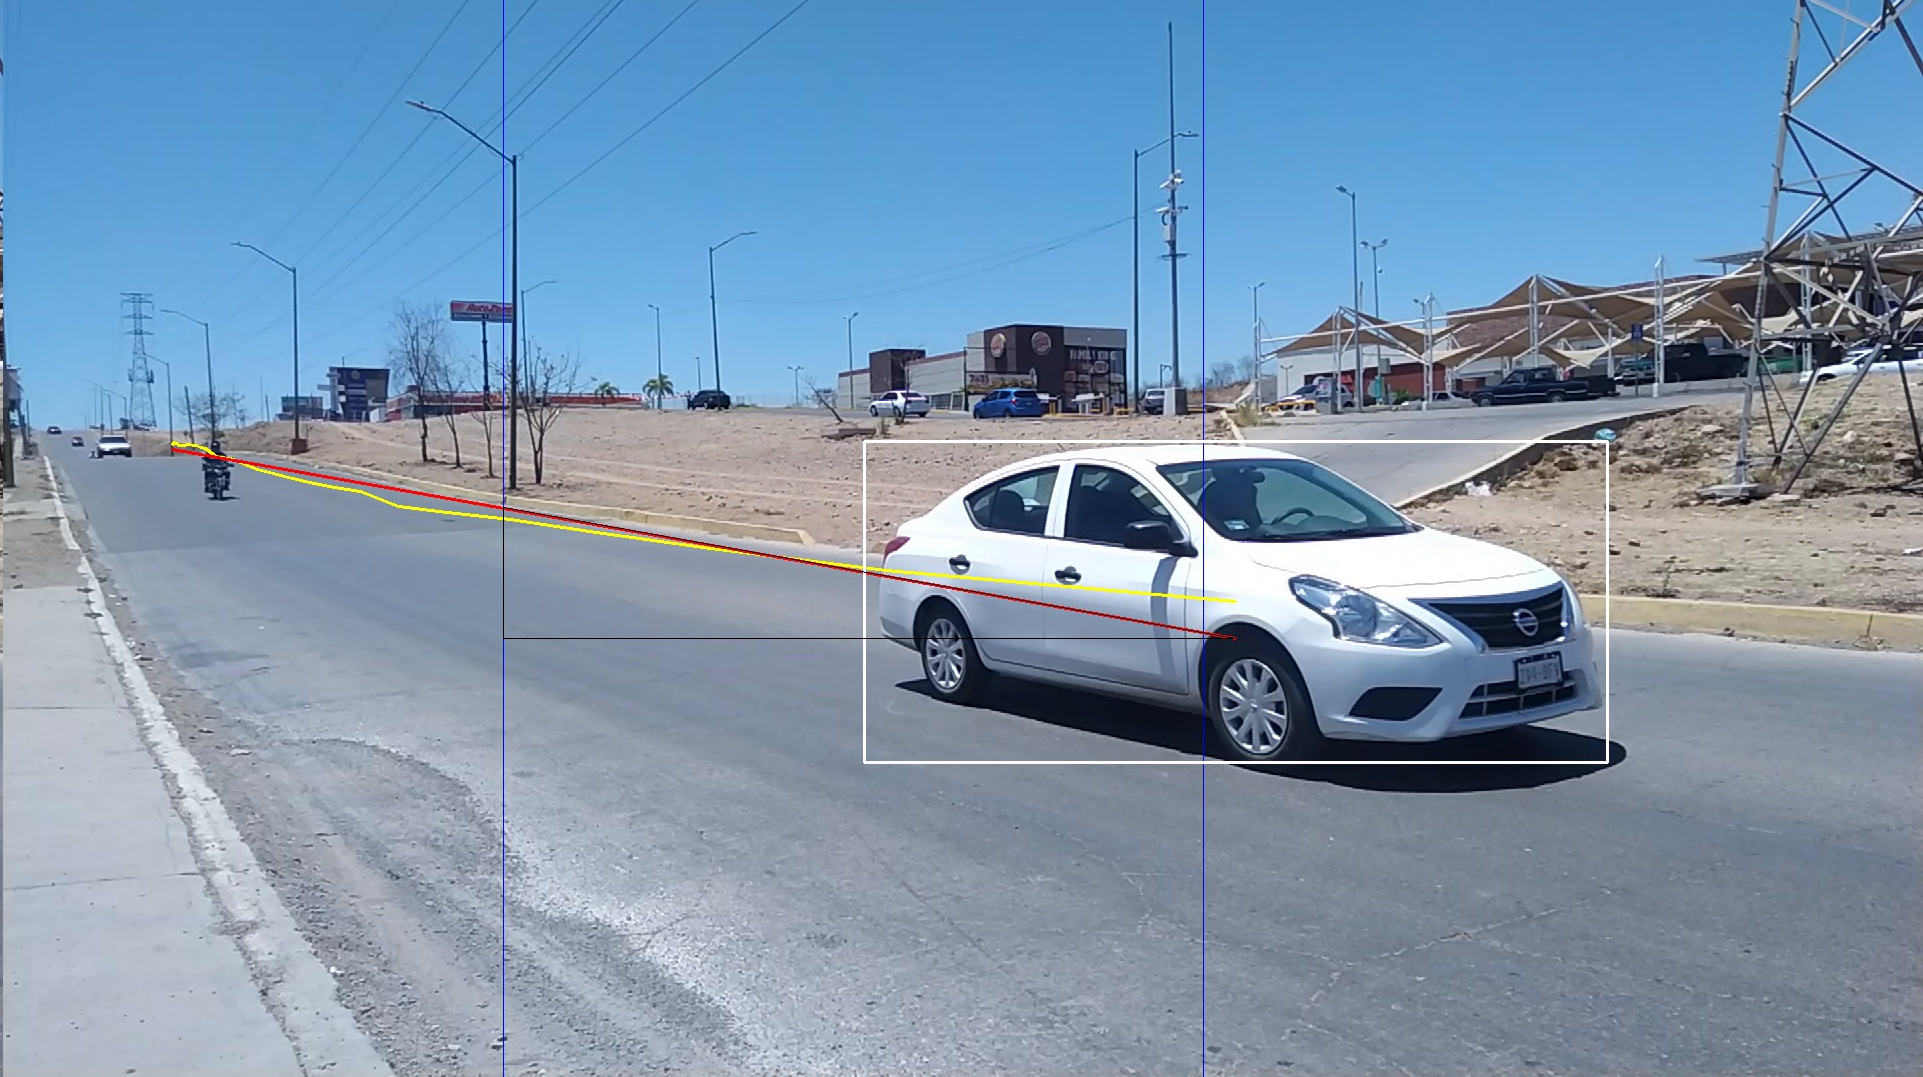
\includegraphics[width=0.8\textwidth]{Metodologia/imgs/Valido_002.jpg}
    \caption{Imagen válida con vehículo saliendo representando una línea del archivo csv.}
    \label{fig:ImagenValida02}
\end{figure}

Por otra parte, hay ocasiones en la cuales el sistema solo detecta parte del vehículo. En este caso la muestra se considera como inválida. Un ejemplo, la Figura \ref{fig:ImagenInvalida_01} muestra el vehículo detectado completamente en el punto A, mientras que cuando el vehículo sale por el punto B es detectado solo una parte (Figura \ref{fig:ImagenInvalida_02}).

\begin{figure}[H]
    \centering
    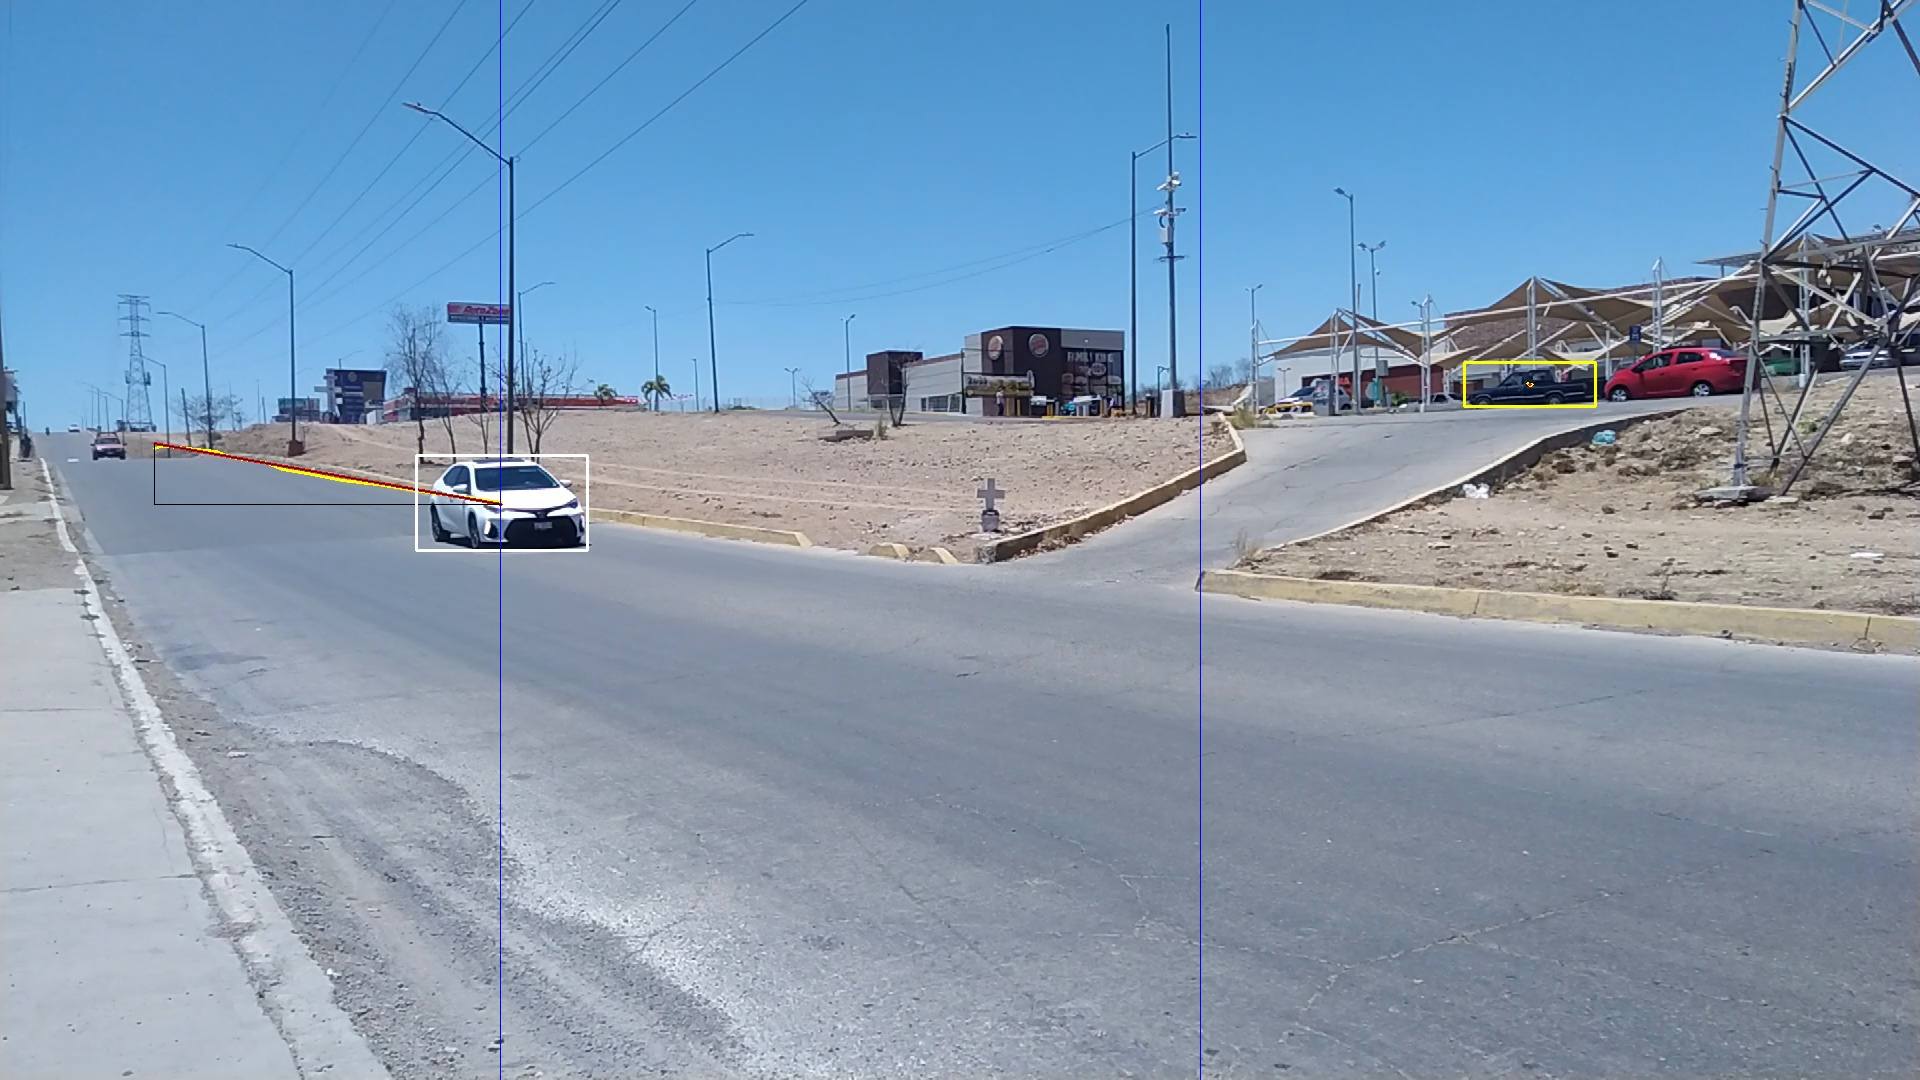
\includegraphics[width=0.8\textwidth]{Metodologia/imgs/Invalido_001.jpg}
    \caption{Imagen inválida (parte izquierda) con vehículo entrando representando una línea del archivo csv.}
    \label{fig:ImagenInvalida_01}
\end{figure}

\begin{figure}[H]
    \centering
    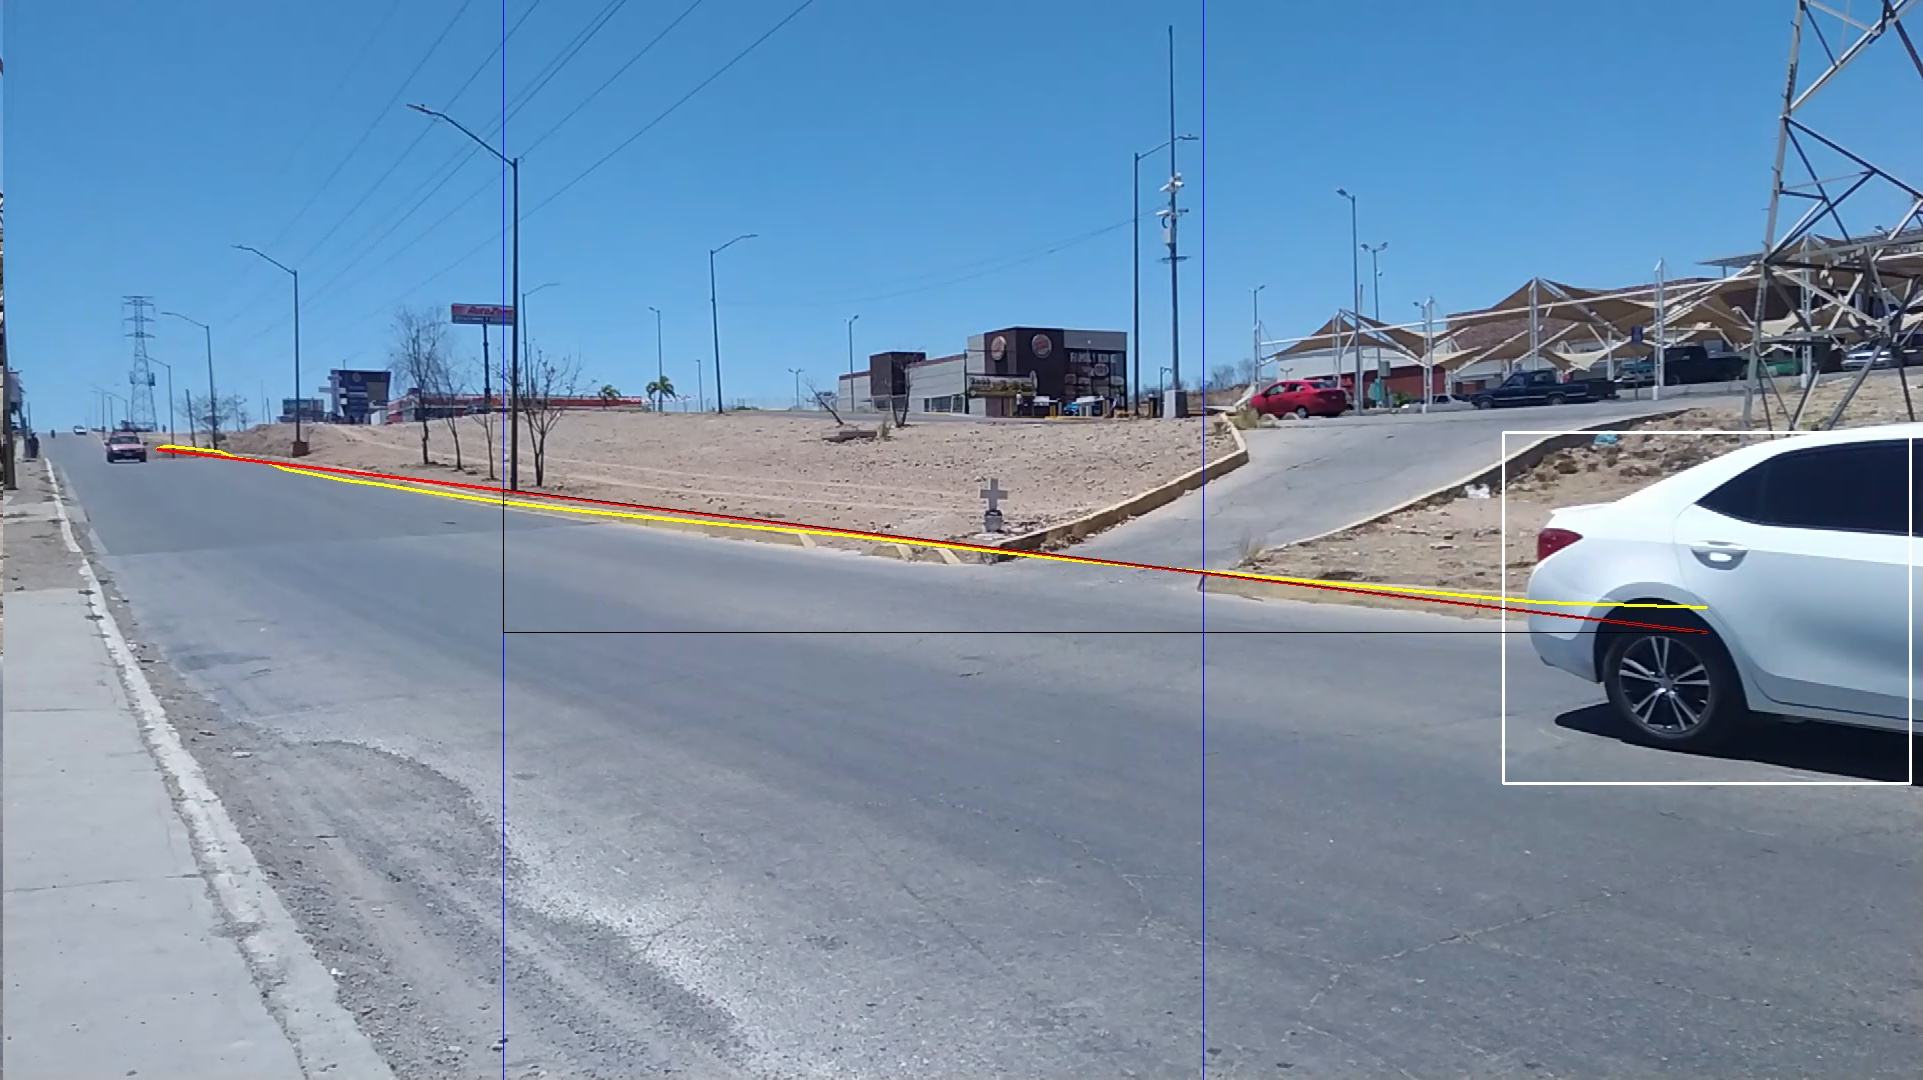
\includegraphics[width=0.8\textwidth]{Metodologia/imgs/Invalido_002.jpg}
    \caption{Imagen inválida (parte derecha) con vehículo saliendo representando una línea del archivo csv.}
    \label{fig:ImagenInvalida_02}
\end{figure}

Una vez que se identifica una imagen inválida se elimina la muestra correspondiente en el archivo csv de salida. Esta muestra se reconoce por el identificador descrito en la Tabla \ref{tab:CaracteristicasSistema}. Para este caso no es necesario volver a ejecutar el sistema.

